\documentclass[11pt,reqno]{amsart}

\usepackage[T1]{fontenc}
\usepackage{amsmath,amssymb,amsthm}
\usepackage{booktabs}
\usepackage{graphicx}
\usepackage[expansion=false]{microtype}
\usepackage{xcolor}
\usepackage[margin=1.2in]{geometry}
\usepackage[colorlinks=true,linkcolor=blue!50!black,citecolor=blue!50!black,
            urlcolor=blue!50!black]{hyperref}

\theoremstyle{plain}
\newtheorem{theorem}{Theorem}[section]
\newtheorem{proposition}[theorem]{Proposition}
\newtheorem{lemma}[theorem]{Lemma}
\newtheorem{corollary}[theorem]{Corollary}
\theoremstyle{definition}
\newtheorem{remark}[theorem]{Remark}

\DeclareMathOperator{\Res}{Res}
\newcommand{\R}{\mathbb{R}}
\newcommand{\C}{\mathbb{C}}
\newcommand{\Rp}{\operatorname{Re}}
\newcommand{\Ip}{\operatorname{Im}}
\newcommand{\lxi}[1]{\left(\tfrac{\xi'}{\xi}\right)\!#1}
\newcommand{\NS}{\mathcal N_{\mathrm S}}

\title[The shifted zeta string]
      {The shifted zeta string: an unconditional\\ inverse-spectral family and its RH endpoint}

% ---------------------------------------------------------------------------

\author{Edward B. Baker III}
\email{edwardbaker86@gmail.com}

\date{\today}

\begin{document}

\begin{abstract}
Suzuki's shifted screw functions $\Psi_\omega$ attach to the Riemann zeta-function, for every
$\omega\ge\tfrac12$ \emph{unconditionally} --- and for every $\omega>\Theta-\tfrac12$ under the
corresponding zero-free half-plane --- a positive inverse-spectral system: a Kre\u\i n string
$S[m_\omega,\infty)$ whose principal Weyl function is
$q_\omega(z)=i(\xi'/\xi)(\tfrac12+\omega-i\sqrt z)/\sqrt z$. We identify its spectral measure in
closed form: it is purely absolutely continuous, and its density is the zero-counting measure of
$\zeta$ smeared by Poisson kernels, each zero $\rho=\beta+i\tau$ contributing a Lorentzian of
width $\tfrac12+\omega-\beta$ centred at $\tau$ --- of width exactly $\omega$ under the Riemann
Hypothesis. Three exact bridges follow. The screw function itself is the spectral transform
$\Psi_\omega(t)=\int_\R(1-\cos ut)u^{-2}\rho_\omega(u)\,du$; consequently the linear margin of
the shifted screw criterion, studied in the companion paper, equals $\pi$ times the spectral
density at zero frequency. The string has a homogeneous infrared bulk whose density is the
inverse square of that margin, $\rho_\infty(\omega)=[(\xi'/\xi)(\tfrac12+\omega)]^{-2}$, and a
universal ultraviolet law $m_\omega(x)\sim4x(\log x)^{-2}$, the unconditional analogue of
Kotani's theorem for his RH-conditional zeta string. Finally, the family detects the zeros
through its existence: $q_\omega$ is a Stieltjes function for every $\omega>0$ if and only if
the Riemann Hypothesis holds --- a zero off the critical line creates non-real poles, destroying
the positive string realisation below the critical shift --- and under RH the family degenerates
at its endpoint onto Kotani's string: the spectral measures converge vaguely, as
$\omega\downarrow0$, to the pure-point measure $2\sum_{\tau>0}\delta_{\tau^2}$, with locally
uniform convergence of Weyl functions at rate $O(\omega)$. The degeneration is geometric as
well as spectral: every $\omega$-string has infinite length, while Kotani's limit string has
finite length $(\xi'/\xi)'(\tfrac12)=0.04620\ldots$. We provide independent numerical checks
of the spectral formulas and compute finite approximations to the associated strings by
discretisation and Herglotz peeling.
\end{abstract}

\maketitle

\setcounter{tocdepth}{1}
\tableofcontents

% ===========================================================================
\section{Introduction}\label{sec:intro}
% ===========================================================================

\subsection{Context}
Suzuki \cite{Suzuki2023} attached to the Riemann zeta-function a continuous real function
$\Psi(t)$ --- the twice-integrated, normalised error term in the prime number theorem --- and
proved that the Riemann Hypothesis (RH) is equivalent to $\Psi\ge0$ pointwise. The mechanism is
the Kre\u\i n--Langer theory of screw functions \cite{KreinLanger}: RH holds if and only if
$Q_\xi(z)=i(\xi'/\xi)(\tfrac12-iz)$ is a Herglotz function (Lagarias \cite{Lagarias1999}), if
and only if $-\Psi$ is a screw function. Under RH, the associated Stieltjes-class function
$q_\xi(z)=Q_\xi(\sqrt z)/\sqrt z$ has the expansion $\sum_{\tau>0}2/(\tau^2-z)$ over the
ordinates of the zeros, and Kre\u\i n's inverse theorem \cite{Krein1952} attaches to it a
string --- Kotani's \emph{zeta string} \cite{Kotani}, with pure point spectral measure of mass
$2$ at each $\tau^2$ and mass function $m_\xi(x)\sim4x(\log x)^{-2}$ as $x\to0^+$
(\cite{Kotani}; see \cite[\S9]{Suzuki2023}).

All of that is conditional: without RH there is no positive object at $\omega=0$. Suzuki also
introduced \cite[\S11]{Suzuki2023} the shifted family $\Psi_\omega$, with
\begin{equation}\label{eq:laplace}
  \int_0^\infty\Psi_\omega(t)\,e^{izt}\,dt
  =-\frac1{z^2}\,\lxi{\left(\tfrac12+\omega-iz\right)},
\end{equation}
and proved that $\xi(s)\neq0$ on $\Rp(s)>\tfrac12+\omega$ if and only if $\Psi_\omega\ge0$
eventually. The companion paper \cite{Margin} makes that criterion quantitative:
unconditionally
\begin{equation}\label{eq:margin}
  \Psi_\omega(t)=\lxi{\left(\tfrac12+\omega\right)}\,t+\lxi{'\left(\tfrac12+\omega\right)}
  +O\!\left(e^{-(\omega-\vartheta)t}\right),\qquad \vartheta=\Theta-\tfrac12,
\end{equation}
with explicit constants; the linear coefficient --- the \emph{margin slope} --- vanishes as
$\omega\to0^+$ precisely because $(\xi'/\xi)(\tfrac12)=0$, which is why RH is the marginal
member of the family. For $\omega\ge\tfrac12$ the criterion is unconditional ---
$\zeta(s)\neq0$ on $\Rp(s)>1$ is the prime number theorem --- and, as recalled in
\cite{Margin}, Suzuki's Herglotz argument then makes $-\Psi_\omega$ a screw function outright.
Combining that shifted Herglotz positivity with Kre\u\i n's correspondence suggests that
$\zeta$ carries, unconditionally, a one-parameter family of positive inverse-spectral systems,
extending Suzuki's construction at $\omega=0$ \cite[\S9]{Suzuki2023}. The present paper
develops that family explicitly.

\subsection{Results}
Fix $\omega\ge\tfrac12$ and write $\sigma=\tfrac12+\omega$. For $z\in\C\setminus[0,\infty)$
take the branch of $\sqrt z$ with $\Ip\sqrt z>0$ and set $w=-i\sqrt z$, so $\Rp w>0$ and
$z=-w^2$. Define
\begin{equation}\label{eq:qdef}
  q_\omega(z):=\frac{(\xi'/\xi)(\sigma+w)}{w}
  =\frac{i}{\sqrt z}\,\lxi{\left(\sigma-i\sqrt z\right)} .
\end{equation}
Zeros of $\xi$ are written $\rho=\beta+i\tau$; sums over $\rho$ count multiplicity. Recall the
Stieltjes class $\NS$: Herglotz functions analytic and non-negative on $(-\infty,0)$, i.e.\
functions of the form $b+\int_0^\infty(\lambda-z)^{-1}d\sigma(\lambda)$ with $b\ge0$ and
$\int(1+\lambda)^{-1}d\sigma<\infty$; Kre\u\i n's correspondence \cite{Krein1952,KacKrein}
attaches to each such function a unique string $S[m,L]$ (a length $0<L\le\infty$ and a
non-decreasing mass function $m$ on $[0,L)$) whose principal Titchmarsh--Weyl function it is.

\begin{theorem}[spectral measure; Section \ref{sec:thmA}]\label{thm:A}
Let $\omega\ge\tfrac12$. Then $q_\omega\in\NS$, with $b=0$, no linear term, and purely
absolutely continuous spectral measure
\begin{equation}\label{eq:measure}
  d\sigma_\omega(\lambda)=\frac{\rho_\omega(\sqrt\lambda)}{\sqrt\lambda}\,d\lambda
  \quad\text{on }[0,\infty),
  \qquad
  \rho_\omega(u)=\frac1\pi\,\Rp\lxi{(\sigma+iu)}
  =\frac1\pi\sum_\rho\frac{\sigma-\beta}{(\sigma-\beta)^2+(u-\tau)^2},
\end{equation}
the sum over all zeros being absolutely convergent. Consequently there is a unique string
$S[m_\omega,L_\omega]$ with principal Weyl function $q_\omega$; it has $L_\omega=\infty$ and
$m_\omega(\infty)=\infty$. The same statements hold for $\omega\in(\vartheta,\tfrac12)$
conditionally on the zero-free half-plane $\Rp(\rho)\le\tfrac12+\vartheta<\sigma$.
\end{theorem}

The density \eqref{eq:measure} is the zero-counting measure smeared by Poisson kernels: each
zero contributes a Lorentzian of width $\sigma-\beta$ --- its distance to the boundary line ---
centred at its ordinate. Under RH every width equals $\omega$ exactly. See
Figure~\ref{fig:density}.

\begin{theorem}[screw representation and the margin identity; Section \ref{sec:thmB}]\label{thm:B}
Let $\omega\ge\tfrac12$ (or $\omega>\vartheta$ conditionally). Then for all $t\ge0$,
\begin{equation}\label{eq:screwrep}
  \Psi_\omega(t)=\int_\R\frac{1-\cos(ut)}{u^2}\,\rho_\omega(u)\,du ,
\end{equation}
absolutely convergent, with exactly the stated normalisation. In particular
\begin{equation}\label{eq:marginident}
  \boxed{\ \lxi{\left(\tfrac12+\omega\right)}=\pi\,\rho_\omega(0)\ }
\end{equation}
--- the margin slope of \cite{Margin} is $\pi$ times the spectral density at zero frequency.
\end{theorem}

\begin{theorem}[infrared bulk; Section \ref{sec:thmCD}]\label{thm:C}
Under the hypotheses of Theorem \ref{thm:A} (in particular, unconditionally for
$\omega\ge\tfrac12$),
\[
  \frac{m_\omega(x)}{x}\;\longrightarrow\;
  \rho_\infty(\omega):=\left[\lxi{\left(\tfrac12+\omega\right)}\right]^{-2}
  \qquad(x\to\infty).
\]
At $\omega=\tfrac12$ the bulk density of the unconditional zeta string is
$(\xi'/\xi)(1)^{-2}=1874.7243\ldots$, with
$(\xi'/\xi)(1)=\tfrac{\gamma_0}2+1-\tfrac12\log4\pi=0.0230957\ldots$.
\end{theorem}

Together, \eqref{eq:marginident} and Theorem \ref{thm:C} give the chain that motivates this
paper:
\[
  \text{margin slope}\;=\;\pi\times(\text{zero-frequency density of states})
  \;=\;\rho_\infty^{-1/2} .
\]
The central quantity of the criterion in \cite{Margin} is, on the string side, the reciprocal
square root of the bulk density.

\begin{theorem}[ultraviolet law; Section \ref{sec:thmCD}]\label{thm:D}
Under the hypotheses of Theorem \ref{thm:A},
\[
  m_\omega(x)\;\sim\;\frac{4x}{(\log x)^2}\qquad(x\to0^+);
\]
in particular this holds unconditionally for every $\omega\ge\tfrac12$, with the same law and
constant as Kotani's RH-conditional zeta string \cite{Kotani}. (The asymptotic computation on
the Weyl-function side is unconditional and $\omega$-independent throughout; only the
existence of the positive string requires the hypothesis.)
\end{theorem}

The last group of results concerns the endpoint $\omega\downarrow0$, and is where the family
sees RH.

\begin{theorem}[existence of the family $\Longleftrightarrow$ RH; Section \ref{sec:thmE}]\label{thm:Eprime}
Let $0<\omega$ and suppose $\xi$ has a zero $\rho=\beta+i\tau$, $\tau>0$, with
$\beta>\sigma=\tfrac12+\omega$. Then $q_\omega$ is meromorphic on $\C\setminus[0,\infty)$ with
the non-real pole pair
\[
  z_\rho=\tau^2-(\beta-\sigma)^2\mp2i\tau(\beta-\sigma)
  \qquad(\text{from } \rho \text{ and } \overline\rho),
\]
hence $q_\omega\notin\NS$ and no positive string realisation exists. Combined with
Theorem \ref{thm:A}:
\[
  \boxed{\ \text{RH}\iff q_\omega\in\NS\text{ for every }\omega>0
  \iff\text{the }\omega\text{-string family extends to all }\omega>0.\ }
\]
\end{theorem}

\begin{theorem}[RH endpoint; Section \ref{sec:thmE}]\label{thm:E}
As $\omega\downarrow0$:
\begin{enumerate}
\item[(i)] Unconditionally, $q_\omega\to q_\xi$, $q_\xi(z)=i(\xi'/\xi)(\tfrac12-i\sqrt z)/\sqrt z$,
locally uniformly on $\C\setminus([0,\infty)\cup P)$, where $P$ is the pole set of $q_\xi$; the
rate is $O(\omega)$, locally uniformly. Under RH, $P\subset[0,\infty)$ and the convergence is
locally uniform on all of $\C\setminus[0,\infty)$.
\item[(ii)] Under RH, the spectral measures converge vaguely to Kotani's pure-point measure:
\[
  \sigma_\omega\;\Longrightarrow\;2\sum_{\tau>0}\delta_{\tau^2}
  \qquad(\omega\downarrow0).
\]
\item[(iii)] Under RH, $m_\omega(x)\to m_\xi(x)$ at every continuity point of $m_\xi$, by
continuity of Kre\u\i n's correspondence \cite[Thm.~1]{Kasahara}.
\end{enumerate}
Without RH, by Theorem \ref{thm:Eprime} the family cannot be continued below
$\omega_c=\Theta-\tfrac12>0$ (for $\omega=\omega_c$ itself see Remark \ref{rem:critical}) and
the endpoint is never reached: the statement ``$\sigma_\omega$ converges, as
$\omega\downarrow0$, to a positive measure'' is itself equivalent to RH at the level of the
family.
\end{theorem}

Under RH the transition at $\omega=0$ is thus an absolutely-continuous-to-pure-point spectral
limit: the Lorentzians of Theorem \ref{thm:A}, all of width exactly $\omega$, sharpen to the
point masses of Kotani's string. The endpoint is singular geometrically as well: every
$\omega$-string has infinite length, while Kotani's limit string has finite length
$(\xi'/\xi)'(\tfrac12)$ (Remark \ref{rem:length}). We do not claim any statement about
eigenfunctions or dynamics, and accordingly avoid the word ``localisation'' except as an
interpretive gloss (Section \ref{sec:physics}).

\subsection{What is new, and what is Suzuki's}
The objects are Suzuki's: the screw function, the shifted family, the Laplace identity
\eqref{eq:laplace}, and, under RH, the identification of $q_\xi$ with Kotani's string
\cite[\S9]{Suzuki2023}; the margin asymptotics \eqref{eq:margin} are from the companion paper
\cite{Margin}. What is offered here is the unconditional inverse-spectral family itself:
the closed-form identification of the spectral measure (Theorem \ref{thm:A}), the exact
normalisation of the spectral representation of $\Psi_\omega$ and the resulting margin identity
(Theorem \ref{thm:B}), the bulk and ultraviolet laws for the string (Theorems \ref{thm:C},
\ref{thm:D}), the equivalence of RH with the existence of the full family and the endpoint
degeneration onto Kotani's string (Theorems \ref{thm:Eprime}, \ref{thm:E}), and the numerical
computation of the strings (Section \ref{sec:numerics}).

\subsection*{Source of the Tauberian input}
Theorems \ref{thm:C} and \ref{thm:D} reduce, after exact computations with $q_\omega$, to
Kasahara's regular-variation theorem for Kre\u\i n's correspondence,
\cite[Thm.~2 and Example~1]{Kasahara}, applied at index $\alpha=\tfrac12$, where his constant
is $D_{1/2}=1$; Theorem \ref{thm:E}(iii) uses his continuity theorem \cite[Thm.~1]{Kasahara}.
We have checked the statements, constants, and endpoint conventions against the original (see
also \cite{KotaniWatanabe,KasaharaWatanabe2009,KasaharaWatanabe2010} and, for canonical
systems, \cite{EKT}). Two convention notes: Kasahara's characteristic function
$h(s)=a+\int_0^\infty(\lambda+s)^{-1}d\sigma(\lambda)$ \cite[(5),(7)]{Kasahara} is
$h(s)=q_\omega(-s)$ in our normalisation; and his mass functions are the left-continuous
representatives \cite[\S1]{Kasahara}, ours right-continuous --- immaterial, since every
statement used below concerns continuity points.

% ===========================================================================
\section{Setup}\label{sec:setup}
% ===========================================================================

Notation follows \cite{Suzuki2023,Margin}: $\xi(s)=\tfrac12s(s-1)\pi^{-s/2}\Gamma(s/2)\zeta(s)$,
entire of order one, $\xi(s)=\xi(1-s)=\overline{\xi(\bar s)}$; zeros $\rho=\beta+i\tau$ with
$0\le\beta\le1$, $|\tau|\ge14.13$; $\Theta=\sup_\rho\beta$, $\vartheta=\Theta-\tfrac12$.
Throughout, $\omega>0$ and $\sigma=\tfrac12+\omega$; the standing hypothesis is
\begin{equation}\label{eq:standing}
  \beta<\sigma\quad\text{for every zero }\rho=\beta+i\tau .
\end{equation}
For $\sigma\ge1$ this holds unconditionally: every individual zero has $\beta<1$ ($\beta\le1$
trivially, and there are no zeros on $\Rp(s)=1$, by Hadamard and de la Vall\'ee Poussin). For
$\sigma<1$ it is the zero-free half-plane hypothesis $\sigma>\Theta$. We emphasise that at
$\sigma=1$ no uniform gap $\inf_\rho(\sigma-\beta)>0$ is asserted --- it is not known that
$\Theta<1$ --- and no proof below requires one: only the pointwise inequality
\eqref{eq:standing} enters.

For strings we use the normalisation of \cite[\S9]{Suzuki2023}: a string $S[m,L]$ is
$0<L\le\infty$ together with a right-continuous non-decreasing $m\ge0$ on $[0,L)$,
$m(0-)=0$; the string equation is $dy'+zy\,dm=0$ with solutions $\varphi(\cdot,z)$,
$\psi(\cdot,z)$ normalised by $\varphi(0)=\psi'(0)=1$, $\varphi'(0)=\psi(0)=0$; the principal
Weyl function is $q(z)=\lim_{x\to L}\psi(x,z)/\varphi(x,z)\in\NS$, and Kre\u\i n's theorem
\cite{Krein1952,KacKrein} says $S[m,L]\mapsto q$ is a bijection onto $\NS$. The model case used
twice below: for $dm=\rho\,dx$ on $[0,\infty)$, $\rho>0$ constant,
\begin{equation}\label{eq:homog}
  \varphi(x,-y)=\cosh(\sqrt{\rho y}\,x),\quad
  \psi(x,-y)=\frac{\sinh(\sqrt{\rho y}\,x)}{\sqrt{\rho y}},\quad
  q(-y)=\frac1{\sqrt{\rho y}}\qquad(y>0).
\end{equation}

Two facts from \cite{Suzuki2023,Margin} are used as inputs. First, the Laplace identity
\eqref{eq:laplace}, valid for $\Ip z>\max(0,\tfrac12-\omega)$ and extending by analytic
continuation to $\Ip z>0$ under \eqref{eq:standing}, since then $\Psi_\omega(t)=O(t)$ by
\eqref{eq:margin}. Second, the Hadamard expansion in the paired form:

\begin{lemma}\label{lem:hadamard}
For $s$ off the zeros,
\[
  \lxi{(s)}=\sum_{\tau>0}\left[\frac1{s-\rho}+\frac1{s-\overline\rho}\right],
\]
the sum over conjugate pairs converging absolutely and locally uniformly, with \emph{no}
additive constant.
\end{lemma}

\begin{proof}
By Hadamard, $(\xi'/\xi)(s)=B+\sum_\rho[(s-\rho)^{-1}+\rho^{-1}]$ with
$B=-\sum_\rho\Rp(1/\rho)$, the last sum paired over conjugates
(\cite[\S12]{Davenport}). Grouping conjugate pairs,
$\sum_{\text{pairs}}(\rho^{-1}+\overline\rho^{\,-1})=\sum_\rho\Rp(1/\rho)$ cancels $B$
exactly. Each paired term is $2(s-\beta)/((s-\beta)^2+\tau^2)=O(|s|/\tau^2)$, and
$\sum\tau^{-2}<\infty$.
\end{proof}

% ===========================================================================
\section{The spectral measure: proof of Theorem \ref{thm:A}}\label{sec:thmA}
% ===========================================================================

The analytic heart is one residue computation, which identifies, pair by pair, the Hadamard
expansion of $q_\omega$ with the Stieltjes transform of the corresponding pair of Poisson
kernels.

\begin{lemma}\label{lem:residue}
Let $a>0$, $\tau\in\R$, $z\in\C\setminus[0,\infty)$, and $w=-i\sqrt z$ as in \eqref{eq:qdef}.
Then
\begin{equation}\label{eq:residue}
  \frac1w\left[\frac1{a+w-i\tau}+\frac1{a+w+i\tau}\right]
  =\frac1\pi\int_\R\left[\frac{a}{a^2+(u-\tau)^2}+\frac{a}{a^2+(u+\tau)^2}\right]
  \frac{du}{u^2-z}.
\end{equation}
\end{lemma}

\begin{proof}
Write $v=\sqrt z$ ($\Ip v>0$). The integrand decays like $u^{-4}$; close the contour in the
upper half $u$-plane. Because $a>0$, the Lorentzian poles $u=\pm\tau+ia$ lie in the
\emph{upper} half-plane and contribute $((\pm\tau+ia)^2-z)^{-1}$; the pole $u=v$ contributes
$(i/v)\,a\,(a^2+(v\mp\tau)^2)^{-1}$. Summing the four residues, both sides of
\eqref{eq:residue} are rational in $(a,\tau,v)$; clearing denominators reduces the identity to
\[
  (a^2+v^2+\tau^2)^2-4v^2\tau^2=(\tau^2-a^2-v^2)^2+4a^2\tau^2
  \quad\bigl(\text{both}=(a^2+v^2)^2+2\tau^2(a^2-v^2)+\tau^4\bigr)
\]
with matching numerators $-2(a^2+v^2-\tau^2)$, an elementary verification. (It was also checked
numerically at four parameter triples, including the near-cut point $z=100+i$, to
$10^{-33}$--$10^{-44}$.)
\end{proof}

\begin{proof}[Proof of Theorem \ref{thm:A}]
\emph{Analyticity and reality.} For $z\in\C\setminus[0,\infty)$ we have $\Rp w>0$, so
$\Rp(\sigma+w)>\sigma$; by \eqref{eq:standing} the open half-plane $\Rp(s)>\sigma$ contains no
zeros, and $q_\omega$ is analytic on the cut plane. On $(-\infty,0)$,
$w=\sqrt{|z|}>0$ and
\begin{equation}\label{eq:qnegaxis}
  q_\omega(-y)=\frac{(\xi'/\xi)(\sigma+\sqrt y)}{\sqrt y}>0\qquad(y>0),
\end{equation}
positivity because each paired Hadamard term $2(s-\beta)/((s-\beta)^2+\tau^2)$ is positive for
real $s\ge\sigma$, by \eqref{eq:standing}.

\emph{The Stieltjes-transform identity.} Apply Lemma \ref{lem:residue} to each conjugate pair,
with $a=\sigma-\beta>0$ --- which is exactly the standing hypothesis \eqref{eq:standing}, and
requires no uniform lower bound. Summing over pairs and using Lemma \ref{lem:hadamard} on
the left,
\begin{equation}\label{eq:stieltjes}
  q_\omega(z)=\int_\R\frac{\rho_\omega(u)}{u^2-z}\,du
  =\int_0^\infty\frac{d\sigma_\omega(\lambda)}{\lambda-z},
\end{equation}
the second equality by $\lambda=u^2$ and evenness of $\rho_\omega$. The interchange of sum and
integral is dominated convergence: $|u^2-z|\ge c_z(1+u^2)$ for fixed $z$ off the cut, and the
convolution of two Poisson kernels being a Poisson kernel,
\[
  \int_\R\frac1\pi\,\frac{a}{a^2+(u-\tau)^2}\cdot\frac{du}{1+u^2}
  =\frac{1+a}{(1+a)^2+\tau^2}=O\!\left(\frac\sigma{\tau^2}\right),
\]
which is summable over the zeros.

\emph{Stieltjes class and the representation.} By \eqref{eq:stieltjes} with $\rho_\omega\ge0$:
$\Ip q_\omega(z)=\Ip z\int\rho_\omega(u)|u^2-z|^{-2}du>0$ on $\C^+$, and $q_\omega>0$ on
$(-\infty,0)$, so $q_\omega\in\NS$. The measure satisfies
$\int(1+\lambda)^{-1}d\sigma_\omega<\infty$: near $0$ the density is
$\sim\rho_\omega(0)/\sqrt\lambda$, integrable; at $\infty$ it is
$O(\log\lambda\cdot\lambda^{-1/2})\cdot\lambda^{-1}$ against $d\lambda$, again integrable,
since $\rho_\omega(u)=O(\log u)$ uniformly for $\sigma\ge1$: by Stirling
$\tfrac12\psi(\tfrac{\sigma+iu}2)=\tfrac12\log\tfrac u2+O(1)$, and
$(\zeta'/\zeta)(\sigma+iu)=O(\log u)$ classically \cite[(3.11.7)]{Titchmarsh}. (For fixed
$\sigma>1$, absolute convergence of the Dirichlet series gives the sharper pointwise
$\rho_\omega(u)=\tfrac1{2\pi}\log\tfrac u{2\pi}+O_\sigma(1)$; uniformly down to $\sigma=1$
only the $O(\log u)$ bound is claimed, and only it is needed. In the mean, $\rho_\omega$
follows the Riemann--von Mangoldt density --- see Figure \ref{fig:density}.) The additive constant is
$b=\lim_{y\to\infty}q_\omega(-y)=0$ by \eqref{eq:largey}, and there is no linear term.

\emph{Absolute continuity.} $\xi'/\xi$ is analytic at every point of the closed half-plane
$\Rp(s)\ge\sigma$: the zeros are discrete, none lies there by \eqref{eq:standing}, and the pole
of $\zeta$ at $s=1$ is cancelled in $\xi$ ($\xi(1)=\tfrac12\neq0$). So $q_\omega$ extends
continuously from $\C^+$ to $(0,\infty)$ with
\[
  \frac1\pi\,\Ip q_\omega(\lambda+i0)
  =\frac1{\sqrt\lambda}\cdot\frac1\pi\Rp\lxi{(\sigma+i\sqrt\lambda)}
  =\frac{\rho_\omega(\sqrt\lambda)}{\sqrt\lambda},
\]
using $w\to-i\sqrt\lambda$ and conjugate symmetry. Stieltjes--Perron inversion on compact
subsets of $(0,\infty)$ identifies $d\sigma_\omega$ with this continuous density; there is no
singular part on $(0,\infty)$, and no atom at $0$ since $q_\omega(z)=O(|z|^{-1/2})$ near $0$
gives $\varepsilon\,|q_\omega(i\varepsilon)|\to0$.

\emph{The string.} Kre\u\i n's theorem \cite{Krein1952,KacKrein} attaches the unique
$S[m_\omega,L_\omega]$. By \eqref{eq:qnegaxis}, $q_\omega(-y)\uparrow\infty$ as $y\downarrow0$
(the transform $\int d\sigma_\omega/(\lambda+y)$ is decreasing in $y$ and diverges, the measure
having a $\lambda^{-1/2}$ density at $0$); since the length is
$L_\omega=\lim_{s\downarrow0}h(s)$ in the Kre\u\i n--Kasahara normalisation
\cite[(9)]{Kasahara}, with $h(s)=q_\omega(-s)$, this gives $L_\omega=\infty$ directly;
and Theorem \ref{thm:C} gives $m_\omega(\infty)=\infty$.
\end{proof}

\begin{remark}[where positivity enters]\label{rem:failure}
The proof localises the role of the zero-free half-plane exactly. If a zero has
$\beta>\sigma$, its Lorentzian pole $u=\tau+i(\sigma-\beta)$ crosses into the \emph{lower} half
$u$-plane and Lemma \ref{lem:residue} acquires a residue correction: $q_\omega$ then equals
$\int\rho_\omega(u)(u^2-z)^{-1}du$ \emph{plus} explicit non-Herglotz pole terms. The boundary
formula for $\rho_\omega$ in \eqref{eq:measure} continues to hold, but $q_\omega$ is no longer
the Stieltjes transform of its own boundary density. This is the mechanism behind Theorem
\ref{thm:Eprime}; whether the density $\rho_\omega$ itself becomes negative somewhere below the
critical shift is a separate question, which we neither need nor claim (a violating zero at
height $\tau$ contributes $-1/(\beta-\sigma)$ at $u=\tau$ against a positive background of
order $\log\tau$).
\end{remark}

% ===========================================================================
\section{The screw representation: proof of Theorem \ref{thm:B}}\label{sec:thmB}
% ===========================================================================

\begin{proof}[Proof of Theorem \ref{thm:B}]
Both sides of \eqref{eq:screwrep} are continuous in $t$ and polynomially bounded: for the right
side, $(1-\cos ut)u^{-2}\le\min(t^2/2,\,2u^{-2})$ and
$\int_\R\min(t^2,u^{-2})\,\rho_\omega(u)\,du<\infty$ since
$\int_{|u|>1}\rho_\omega(u)u^{-2}du<\infty$; for the left side this is \eqref{eq:margin}. So
both Laplace transforms converge on $\Ip z>0$, and by uniqueness of Laplace transforms of
continuous polynomially bounded functions it suffices to match them. The left transform is
\eqref{eq:laplace}. For the right, Fubini (justified by the same $\min$-bound against
$e^{-t\Ip z}$) and the elementary transform
\[
  \int_0^\infty(1-\cos ut)\,e^{izt}\,dt=\frac{-iu^2}{z(z^2-u^2)}\qquad(\Ip z>0)
\]
give
\[
  \int_0^\infty\!\!\left[\int_\R\frac{1-\cos ut}{u^2}\rho_\omega(u)\,du\right]e^{izt}dt
  =\frac iz\int_\R\frac{\rho_\omega(u)}{u^2-z^2}\,du
  =\frac iz\,q_\omega(z^2),
\]
by \eqref{eq:stieltjes} at $Z=z^2\in\C\setminus[0,\infty)$. For $\Ip z>0$ the principal upper
root of $z^2$ is $z$ itself, so by \eqref{eq:qdef}
$q_\omega(z^2)=(\xi'/\xi)(\sigma-iz)/(-iz)$, and the transform equals
$-z^{-2}(\xi'/\xi)(\sigma-iz)$ --- identical to \eqref{eq:laplace}.

The margin identity \eqref{eq:marginident} is then immediate: $\rho_\omega(0)=
\pi^{-1}(\xi'/\xi)(\sigma)$, since $\xi'/\xi$ is real at real arguments. Its content is
Theorem \ref{thm:A}: the function whose value at $0$ is the margin slope is \emph{the} spectral
density of the string.
\end{proof}

\begin{remark}
The normalisation in \eqref{eq:screwrep} is fixed twice over: by the transform computation
above, and independently by a numerical comparison against Suzuki's arithmetic (prime-side)
formula for $\Psi_{1/2}$ \cite[\S11]{Suzuki2023}, which agrees to relative accuracy
$1.3\cdot10^{-6}$ at $t=2$ (Section \ref{sec:numerics}). Note also that ``zero-frequency
density'' in \eqref{eq:marginident} refers to the density $\rho_\omega$ on the frequency line
$u$; in the spectral variable $\lambda=u^2$ the density diverges as
$\rho_\omega(0)/\sqrt\lambda$.
\end{remark}

% ===========================================================================
\section{Bulk and ultraviolet laws: proofs of Theorems \ref{thm:C} and \ref{thm:D}}
\label{sec:thmCD}
% ===========================================================================

Both proofs consist of an exact asymptotic computation on the Weyl function --- available in
closed form by \eqref{eq:qnegaxis} --- followed by Kasahara's regular-variation theorem for
Kre\u\i n's correspondence, \cite[Thm.~2]{Kasahara}, applied at index $\alpha=\tfrac12$. We
use his part (iii): for $0<\alpha\le1$ and $L$ continuous, slowly varying at $\infty$ $[0]$,
with $t^\alpha L(t)$ increasing for large [small] $t$ and inverse function $f_\alpha$, the
asymptotic $h(s)\sim D_\alpha s^{-\alpha}L(1/s)$ as $s\to0^+$ $[\infty]$ is equivalent to
$m(x)\sim x^{1/\alpha-1}K_\alpha(x)$ as $x\to\infty$ $[0^+]$, where
$K_\alpha(x)=x^{-1/\alpha}f_\alpha(x)$ is slowly varying and $D_\alpha$ is the constant of his
Example~1 --- at $\alpha=\tfrac12$, $D_{1/2}=\{\tfrac14\}^{-1/2}\Gamma(\tfrac32)/\Gamma(\tfrac12)=1$.
Here $h(s)=q_\omega(-s)$ is the characteristic function of $m_\omega$ \cite[(5),(7)]{Kasahara}.

\begin{proof}[Proof of Theorem \ref{thm:C}]
From \eqref{eq:qnegaxis},
\[
  q_\omega(-y)\,\sqrt y=\lxi{(\sigma+\sqrt y)}
  \;\longrightarrow\;\lxi{(\sigma)}>0\qquad(y\downarrow0),
\]
with error $O(\sqrt y)$; positivity of the limit is Lemma \ref{lem:hadamard} under
\eqref{eq:standing} (quantitatively, for $0<\omega<\tfrac12$,
$(\xi'/\xi)(\sigma)\ge(2+\gamma_0-\log4\pi)\,\omega$ \cite[Cor.~3.1]{Margin}). So the
characteristic function satisfies $h(s)=q_\omega(-s)\sim D_{1/2}\,s^{-1/2}L(1/s)$ as
$s\downarrow0$, with $D_{1/2}=1$ and the constant slowly varying function
$L\equiv c:=(\xi'/\xi)(\sigma)$; $t^{1/2}L(t)=c\sqrt t$ is increasing, so the hypotheses of
\cite[Thm.~2]{Kasahara} hold at its unbracketed ($s\to0^+$, $x\to\infty$) endpoint. Part
(iii), (A)$\Leftrightarrow$(C), gives
\[
  m_\omega(x)\sim x\,K_{1/2}(x)\quad(x\to\infty),
  \qquad
  K_{1/2}(x)=x^{-2}f_{1/2}(x)=x^{-2}\,(x/c)^2=c^{-2},
\]
$f_{1/2}$ being the inverse of $t\mapsto c\sqrt t$. Hence $m_\omega(x)/x\to c^{-2}$. (Sanity
check: for the homogeneous string \eqref{eq:homog} both asymptotics are identities, consistent
with $D_{1/2}=1$.) The numerical value at $\omega=\tfrac12$ uses the classical
$(\xi'/\xi)(1)=-(\xi'/\xi)(0)=\tfrac{\gamma_0}2+1-\tfrac12\log4\pi$.
\end{proof}

\begin{proof}[Proof of Theorem \ref{thm:D}]
At the other end, for $y\to\infty$,
\begin{equation}\label{eq:largey}
  \lxi{(\sigma+\sqrt y)}
  =\tfrac12\psi\!\left(\tfrac{\sigma+\sqrt y}2\right)-\tfrac12\log\pi+O(y^{-1/2})
  =\tfrac14\log y\,\bigl(1+O(1/\log y)\bigr),
\end{equation}
since $(\zeta'/\zeta)(\sigma+\sqrt y)=O(2^{-\sqrt y})$; note the leading term is
\emph{$\omega$-independent and unconditional} --- this is the analytic face of the fact that
the Riemann--von Mangoldt density does not see the shift. Hence the characteristic function
satisfies $h(s)=q_\omega(-s)\sim D_{1/2}\,s^{-1/2}L(1/s)$ as $s\to\infty$, with $D_{1/2}=1$ and
$L(t)=\tfrac14\log(1/t)$: $L$ is continuous and slowly varying at $0$, and
$t^{1/2}L(t)=\tfrac14\sqrt t\log(1/t)$ is increasing for small $t$, so the hypotheses of
\cite[Thm.~2]{Kasahara} hold at its bracketed ($s\to\infty$, $x\to0^+$) endpoint. Part (iii),
(A)$\Leftrightarrow$(C), gives $m_\omega(x)\sim x\,K_{1/2}(x)$ as $x\to0^+$, with
$K_{1/2}(x)=x^{-2}f_{1/2}(x)$ and $f_{1/2}$ the inverse, near $0$, of
$t\mapsto\tfrac14\sqrt t\log(1/t)$. Inverting,
\[
  \sqrt{f_{1/2}(x)}
  =\frac{4x}{\log\bigl(1/f_{1/2}(x)\bigr)}
  \sim\frac{2x}{\log(1/x)},
  \qquad\text{so}\qquad
  f_{1/2}(x)\sim\frac{4x^2}{(\log x)^2},
  \quad
  K_{1/2}(x)\sim\frac4{(\log x)^2},
\]
and $m_\omega(x)\sim4x/(\log x)^2$. The constant agrees with Kotani's RH-conditional case
\cite{Kotani} because only the leading Riemann--von Mangoldt growth of the spectral measure
enters, and that is the same for $\sigma_\omega$ as for Kotani's pure-point measure.
\end{proof}

\begin{remark}[the ultraviolet law is invisible to feasible numerics]\label{rem:UVnumerics}
On the analytic dual curve at $\omega=\tfrac12$, the ratio of $M(y)$ to $4x/(\log x)^2$ (at
$x=q(-y)$) is
\[
  374,\quad 4.26,\quad 1.388,\quad 1.093,\quad 1.008,\quad 0.974
  \qquad\text{at } y=1,\,10^3,\,10^6,\,10^9,\,10^{12},\,10^{15},
\]
tending to $1$ non-monotonically, with slowly varying correction
$\bigl[(\tfrac12\log y-\log(\xi'/\xi))/(\tfrac12\log y-\log2\pi)\bigr]^2$. Probing $y=10^{12}$
requires resolving the spectral measure to $u\sim10^6$; no string reconstruction of feasible
size sees this regime, which is why Theorem \ref{thm:D} is an analytic statement and the
numerics of Section \ref{sec:numerics} validate only the crossover and bulk regions.
\end{remark}

% ===========================================================================
\section{The endpoint: proofs of Theorems \ref{thm:Eprime} and \ref{thm:E}}\label{sec:thmE}
% ===========================================================================

\begin{proof}[Proof of Theorem \ref{thm:Eprime}]
$q_\omega(z)=(\xi'/\xi)(\sigma+w)/w$ has a pole wherever $\sigma+w=\rho$, i.e.\
$w=(\beta-\sigma)+i\tau$, which lies in the admissible half-plane $\Rp w>0$ exactly when
$\beta>\sigma$. Then $z=-w^2=\tau^2-(\beta-\sigma)^2-2i\tau(\beta-\sigma)$, which is non-real
for $\tau\neq0$ (and there are no real zeros of $\xi$); the conjugate zero
$\overline\rho$ gives the conjugate pole. A Herglotz function is analytic off $\R$, so a
non-real pole in the cut plane already excludes $q_\omega$ from the Herglotz class, a fortiori
from $\NS$; by Kre\u\i n's bijection no string has $q_\omega$ as Weyl function. The displayed
equivalence combines this with the conditional case of Theorem \ref{thm:A}: RH gives
\eqref{eq:standing} for every $\omega>0$; conversely, a zero with $\beta>\tfrac12$ destroys
$\NS$ for every $\omega<\beta-\tfrac12$. At $\omega=\omega_c$ itself the family survives; see
Remark \ref{rem:critical}.
\end{proof}

\begin{remark}[the critical member]\label{rem:critical}
Theorem \ref{thm:Eprime} says the family cannot be continued \emph{below}
$\omega_c=\Theta-\tfrac12$; at $\omega=\omega_c$ it still exists. If the supremum $\Theta$ is
not attained, every zero satisfies $\beta<\sigma_c=\tfrac12+\omega_c$, hypothesis
\eqref{eq:standing} holds, and Theorem \ref{thm:A} applies verbatim. If it is attained, the
extremal zeros sit on the boundary line and contribute \emph{real} poles on the cut --- which a
Stieltjes function is permitted to have: the contribution of a boundary pair
$\{\sigma_c+i\tau,\,\sigma_c-i\tau\}$ of multiplicity $m$ to the paired Hadamard expansion of
$q_{\omega_c}$ is exactly
\[
  \frac mw\left[\frac1{w-i\tau}+\frac1{w+i\tau}\right]
  =\frac{2m}{w^2+\tau^2}
  =\frac{2m}{\tau^2-z},
\]
a point mass $2m$ at $\lambda=\tau^2$ --- the degenerate $a\to0^+$ case of Lemma
\ref{lem:residue}, with the same mass normalisation as Kotani's string. The critical member is
thus a string whose spectral measure carries point masses $2m_\rho$ at the squared ordinates of
the extremal zeros, embedded in the absolutely continuous background of the remaining zeros.
(Consistently, on the time side the shifted criterion also survives at the critical shift
\cite{Margin}.) Moreover, for $\omega_c>0$ the bulk and ultraviolet laws persist at
criticality: the closed form \eqref{eq:qnegaxis} is unchanged at $\omega=\omega_c$, and
$(\xi'/\xi)(\sigma_c)>0$ still --- an extremal pair contributes $0$ to the paired Hadamard sum
at real $\sigma_c$, while its mirror pair on $\Rp(s)=1-\sigma_c$ contributes
$4\omega_c/(4\omega_c^2+\tau^2)>0$ --- so the proofs of Theorems \ref{thm:C} and \ref{thm:D}
apply verbatim to the critical string:
$m_{\omega_c}(x)\sim[(\xi'/\xi)(\sigma_c)]^{-2}x$ at infinity and $\sim4x/(\log x)^2$ at $0$.
The distinction at criticality is thus purely one of spectral type --- absolutely continuous,
versus absolutely continuous plus embedded atoms. (The case $\omega_c=0$, where the mirror
symmetry makes the slope vanish, is genuinely different: see Remark \ref{rem:length}.) The
finer structure of the critical string is left as an open problem (Section \ref{sec:open}).
\end{remark}

\begin{proof}[Proof of Theorem \ref{thm:E}]
(i) For $K\subset\C\setminus([0,\infty)\cup P)$ compact, the $w$-image of $K$ has
$\Rp w\ge\delta(K)>0$, so for $0\le\omega\le\omega_0$ the arguments $\sigma+w$ range in a fixed
compact set on which $\xi'/\xi$ is analytic (avoiding, by the definition of $P$, the finitely
many relevant zeros). Then, by the fundamental theorem of calculus along the real segment
from $\tfrac12+w$ to $\tfrac12+\omega+w$,
\[
  q_\omega(z)-q_\xi(z)=\frac1w\int_0^\omega\lxi{'\left(\tfrac12+t+w\right)}dt,
  \qquad\text{whence}\qquad
  \bigl|q_\omega(z)-q_\xi(z)\bigr|
  \le\frac{\omega}{\inf_{z\in K}|w|}\,
  \sup_{\substack{z\in K\\ 0\le t\le\omega_0}}
  \left|\lxi{'\left(\tfrac12+t+w\right)}\right|,
\]
the locally uniform $O(\omega)$ rate. (The integral form is used because the one-variable
mean value theorem is not available for complex-valued functions.) Under RH, every pole of $q_\xi$ sits at $z=\tau^2\in[0,\infty)$
(as $w=i\tau$ has $\Rp w=0$), so $P\subset[0,\infty)$.

(ii) Under RH, \eqref{eq:measure} reads
$\rho_\omega(u)=\tfrac1\pi\sum_\tau\omega/(\omega^2+(u-\tau)^2)$, the sum over all ordinates
(both signs): the density is the Poisson broadening of the zero set, and the claim is the
approximate-identity limit, summed over the zeros. Let $f\in C_c(\R)$ with
$\operatorname{supp}f\subset[-R,R]$. Each term satisfies
$\int_\R P_\omega(u-\tau)f(u)\,du\to f(\tau)$ as $\omega\downarrow0$, where $P_\omega$ is the
unit-mass Poisson kernel. The terms are dominated, uniformly in $0<\omega\le1$, by
$\min\bigl(\|f\|_\infty,\,\pi^{-1}\|f\|_{L^1}\,d(\tau)^{-2}\bigr)$ with
$d(\tau)=\operatorname{dist}(\tau,[-R,R])$, which is summable over the zeros: only finitely
many ordinates have $d(\tau)\le1$, and $\sum\tau^{-2}<\infty$. Dominated convergence for the
series gives $\int f\,d\mu_\omega\to\sum_\tau f(\tau)$, i.e.\
$\mu_\omega\to\sum_\tau\delta_\tau$ vaguely on $\R$; pushing forward under $u\mapsto u^2$
(for $g\in C_c([0,\infty))$, $g(u^2)\in C_c(\R)$) yields
$\sigma_\omega\Rightarrow\sum_\tau\delta_{\tau^2}=2\sum_{\tau>0}\delta_{\tau^2}$, which is
Kotani's measure with its normalisation \cite[\S9]{Suzuki2023}. (One may instead argue
abstractly from (i) via convergence theorems for Herglotz functions, but these require care
here, both measures having infinite total mass; the direct proof makes the sharpening of the
Lorentzians literally the mechanism.)

(iii) Kasahara's continuity theorem \cite[Thm.~1]{Kasahara} states that, for strings $m_n$
with characteristic functions $h_n(s)=q_n(-s)$, convergence $m_n(x)\to m_0(x)$ at every
continuity point of $m_0$ is equivalent to $h_n(s)\to h_0(s)$ for every $s>0$. By (i) and RH,
$q_\omega(-s)\to q_\xi(-s)$ for every $s>0$ --- the negative axis lies in
$\C\setminus[0,\infty)$, away from the poles of $q_\xi$ --- along every sequence
$\omega_n\downarrow0$; hence $m_\omega(x)\to m_\xi(x)$ at every continuity point of $m_\xi$.
(Kasahara works with left-continuous mass functions \cite[\S1]{Kasahara}, ours are
right-continuous; the representatives agree off the countable jump set, and the statement
concerns continuity points only.)
\end{proof}

\begin{remark}
Vague (local weak) convergence is the correct topology in (ii): both $\sigma_\omega$ and the
limit have infinite total mass, and mass escapes to $\lambda=\infty$ under any global weak
formulation. Quantitatively, the convergence in (i) is measured (Section \ref{sec:numerics})
as exactly linear in $\omega$ over $\omega\in[0.01,0.5]$ at fixed test points, and in (ii) a
unit Gaussian test function centred at the first ordinate is captured to $1-O(\omega)$.
\end{remark}

\begin{remark}[the endpoint length collapse]\label{rem:length}
The length of the string detects the endpoint as sharply as the spectral type. For every
$\omega>0$, $L_\omega=\lim_{s\downarrow0}q_\omega(-s)=\infty$ (Theorem \ref{thm:A}(iv), via
\cite[(9)]{Kasahara}), because $(\xi'/\xi)(\sigma)>0$. Under RH, at the endpoint itself the
same formula gives, by the oddness of $\xi'/\xi$ about $\tfrac12$,
\[
  q_\xi(-s)=\frac{(\xi'/\xi)(\tfrac12+\sqrt s)}{\sqrt s}
  \;\longrightarrow\;\lxi{'\left(\tfrac12\right)}=B(0)
  \qquad(s\downarrow0),
\]
so Kotani's string has \emph{finite} length
\[
  L_\xi=B(0)=\sum_\gamma\gamma^{-2}=0.0462099862\ldots
\]
--- the margin-scale constant of \cite[Rem.~2.3]{Margin}; equivalently
$L_\xi=q_\xi(0^-)=\sum_{\tau>0}2/\tau^2$ from Suzuki's expansion \cite[\S9]{Suzuki2023}
(numerically, $q_\xi(-10^{-10})=0.0462099862$). Under RH the $\omega\downarrow0$ limit is
therefore doubly singular: the spectrum degenerates from absolutely continuous to pure point,
and the geometry collapses from infinite-length strings of homogeneous bulk density
$[(\xi'/\xi)(\tfrac12+\omega)]^{-2}\sim(B(0)\,\omega)^{-2}$ to a finite string of length
$B(0)$. The infinitely dense bulk does not persist in the limit: in the inextensible
normalisation $m_\xi\equiv\infty$ on $(B(0),\infty)$, so Theorem \ref{thm:E}(iii) forces
$m_\omega(x)\to\infty$ for every $x>B(0)$ --- the bulk mass is expelled beyond the finite
length as $\omega\downarrow0$.
\end{remark}

% ===========================================================================
\section{Numerical computation of the strings}\label{sec:numerics}
% ===========================================================================

All computations are in \texttt{mpmath}; scripts are available from the author. Six independent
checks of Theorem \ref{thm:A} were run: the closed form of $\rho_\omega$ against the Lorentzian
zero-sum (1000 zeros plus a Riemann--von Mangoldt tail; relative difference
$10^{-5}$--$10^{-7}$); against the prime side of $\xi'/\xi$ at $\sigma=2$ ($2\cdot10^{-7}$);
positivity on $u\in[0,200]$ at $\omega=\tfrac12$ (minimum $=\rho_{1/2}(0)=0.0073516$ at $u=0$);
the integrated density against the Riemann--von Mangoldt count ($\int_0^{100}\rho_{1/2}=29.111$
vs.\ $N(100)=29.002$ --- agreement at the smearing level; the integrated spectral measure has
the same leading growth $\frac u{2\pi}\log\frac u{2\pi e}$ as the zero-counting function);
identity \eqref{eq:screwrep} against Suzuki's arithmetic $\Psi_{1/2}$ ($1.3\cdot10^{-6}$ at
$t=2$); and \eqref{eq:stieltjes} at complex test points ($4\cdot10^{-7}$). The residue identity
\eqref{eq:residue} was verified separately to $10^{-33}$--$10^{-44}$.

\begin{figure}[htbp]
\centering
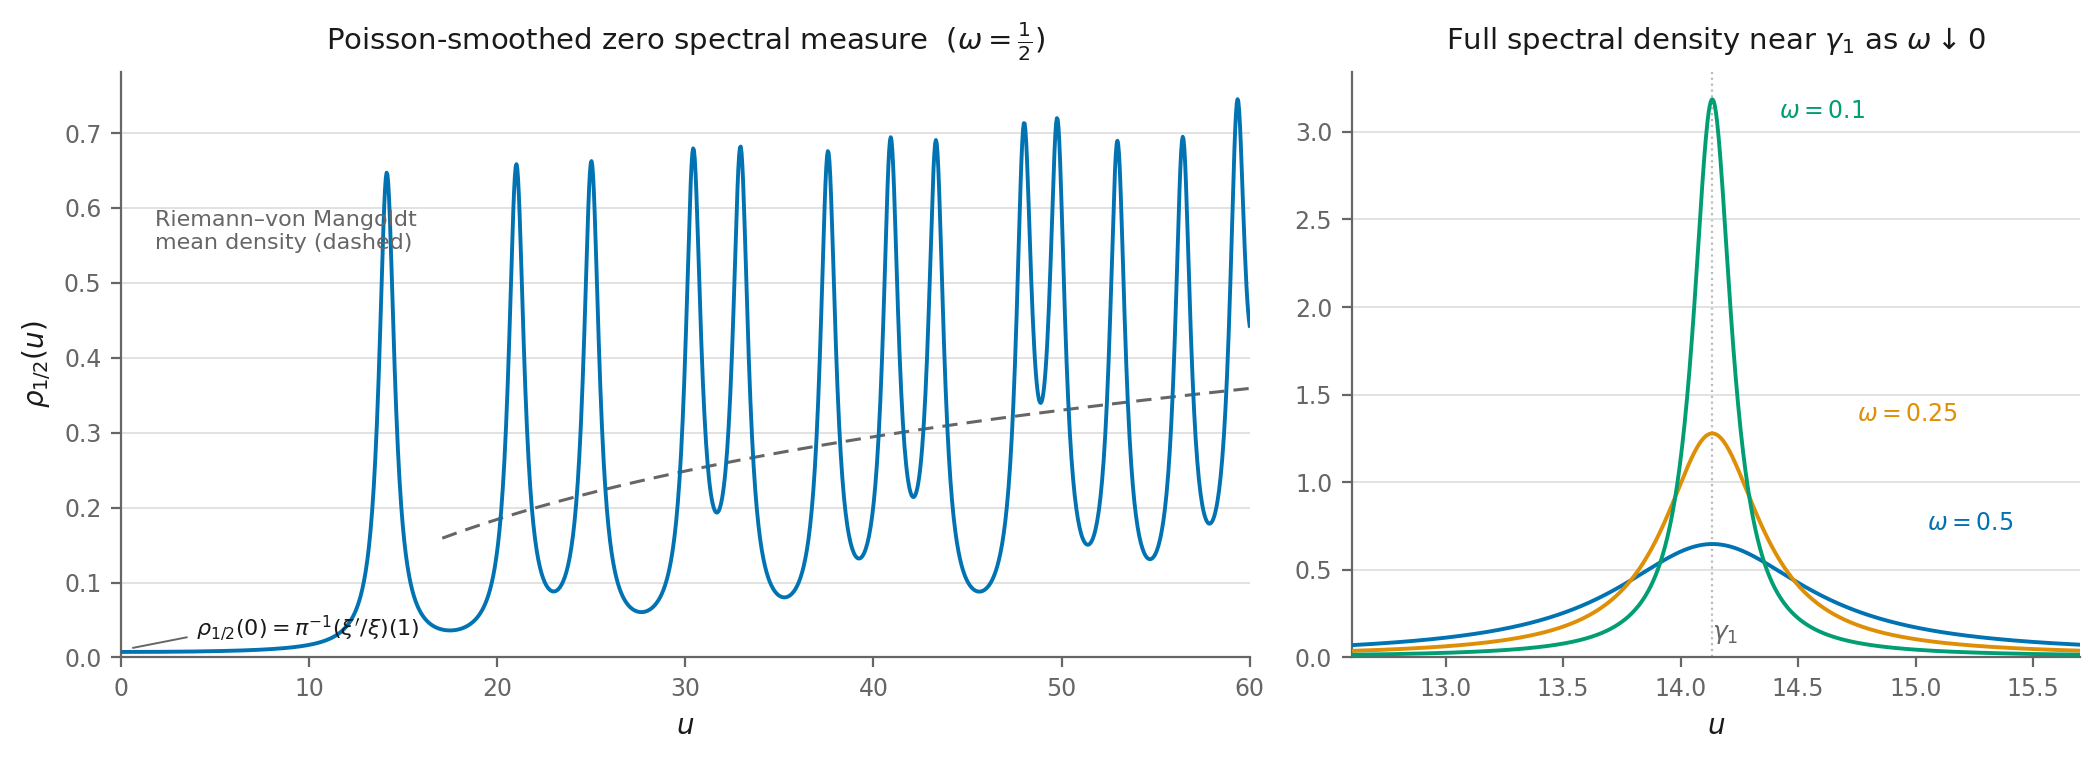
\includegraphics[width=\textwidth]{fig_density.png}
\caption{The Poisson-smoothed zero spectral measure. Left: the density $\rho_{1/2}(u)$ of
\eqref{eq:measure} on $0\le u\le60$ (solid), against the Riemann--von Mangoldt mean density
$\tfrac1{2\pi}\log\tfrac u{2\pi}$ (dashed). Under RH each zero contributes a Lorentzian of
width $\omega$; for the plotted low zeros this is unconditionally valid, their critical-line
location being verified \cite{PlattTrudgian}. The zero-frequency value is the margin slope of
\cite{Margin} divided by $\pi$ (Theorem \ref{thm:B}). Right: the full closed-form density
$\rho_\omega(u)$ near the first ordinate for $\omega=0.5,\,0.25,\,0.1$, sharpening toward the
point mass of Kotani's string as $\omega\downarrow0$ (Theorem \ref{thm:E}); the curves are
visually indistinguishable from the first zero's own Poisson kernel because the background of
all other zeros contributes only $0.011$, $0.005$, $0.002$ at the peak (against peak values
$0.647$, $1.279$, $3.185$; the bare kernel peaks at $1/\pi\omega$). For $\omega<\tfrac12$ the
local picture at this zero is unconditional --- its critical-line location is verified --- but
the interpretation of $\rho_\omega$ as the spectral density of a positive string at those
shifts is conditional (Theorem \ref{thm:Eprime}).}
\label{fig:density}
\end{figure}

\subsection{The discrete inverse problem}
The measure $d\sigma_\omega$ is discretised by Gauss--Legendre panels ($\le152$ point masses up
to a spectral cutoff), and the unique finite Stieltjes string with the resulting rational Weyl
function is recovered by Herglotz peeling --- repeatedly stripping the leading mass and length
read off the large-$y$ behaviour and passing to the inverted remainder, with bracketed
root-finding (one root per gap, guaranteed by interlacing) at $90$--$120$ decimal digits.
Validation: synthetic round trips are exact to $10^{-121}$, and every production string
reproduces its target $q$ at complex test points to $\le10^{-117}$, with all masses and lengths
positive. We emphasise the scope of these figures: they certify the solution of the
\emph{discrete} inverse problem --- the inversion of the finite discretised measure --- to
essentially exact precision. The distance from the finite string to the continuum
$\zeta$-string is a separate, quadrature-dominated question, which the flat-control comparison
below is designed to cancel to leading order.

\subsection{Infrared bulk}
Raw secant fits of $x/m_\omega^{-1}$ deep in the reconstructed bulk give
\[
  \frac{\text{fitted }\rho_\infty}{\text{predicted }(\xi'/\xi)(\sigma)^{-2}}
  =1.30760,\ 1.30774,\ 1.30776
  \qquad\text{at }\omega=0.5,\ 0.75,\ 1.0 :
\]
the $\omega$-scaling of Theorem \ref{thm:C} holds to $\sim10^{-4}$, and the common factor
$1.308$ is discretisation bias, measured on an exactly solvable homogeneous control string
discretised on the same grid as $1.30826$. Control-corrected absolute agreement:
$0.9995,\ 0.9996,\ 0.9996$. This is validation of Theorem \ref{thm:C}, not its proof.
At $\omega=\tfrac12$ the predicted unconditional bulk density is
$\rho_\infty=1874.7243\ldots$.

\subsection{Profile}
The bias-cancelled ratio $m_\zeta(x)/m_{\mathrm{flat}}(x)$ rises from $\approx0$ in a light,
Kotani-type ultraviolet region, through an arithmetic crossover at $x\approx0.05$--$1$ --- dual
to the lowest zeros, $x\sim q(-\tau_1^2)\approx0.05$ --- to the homogeneous bulk (equal to $1$
within $10^{-3}$ for $x\gtrsim3$). The crossover location is the one feature of the profile
with a clean analytic anchor; the ultraviolet law itself is not numerically reachable
(Remark \ref{rem:UVnumerics}).

% ===========================================================================
\section{The physics dictionary}\label{sec:physics}
% ===========================================================================

The mathematics above supports the following dictionary, stated last deliberately; entries are
labelled by their standing.

\begin{itemize}
\item[\emph{(thm)}] Zeros $\leftrightarrow$ resonant spectral locations: each zero is a
Lorentzian resonance of the density of states, of width its distance to the boundary line ---
width exactly $\omega$ under RH (Theorem \ref{thm:A}).
\item[\emph{(thm)}] $\omega$ $\leftrightarrow$ broadening/damping scale; the margin slope of
\cite{Margin} $\leftrightarrow$ $\pi\times$ zero-frequency density of states (Theorem
\ref{thm:B}).
\item[\emph{(thm)}] Bulk string density $\leftrightarrow$ inverse square of the margin slope
(Theorem \ref{thm:C}): the central quantity of the shifted screw criterion is, on the string,
the infrared bulk density --- equivalently, the margin slope is the bulk ``sound speed''
$\rho_\infty^{-1/2}$.
\item[\emph{(thm)}] $\omega\downarrow0$ under RH $\leftrightarrow$ an
absolutely-continuous-to-pure-point spectral limit onto Kotani's string (Theorem \ref{thm:E});
$\rho_\infty\sim\bigl(B(0)\,\omega\bigr)^{-2}\to\infty$: the bulk becomes infinitely heavy ---
and simultaneously the geometry collapses, $L_\omega=\infty$ for every $\omega>0$ while
$L_\xi=B(0)<\infty$ (Remark \ref{rem:length}): the limit is not an infinitely dense infinite
bulk, but a finite string of length $B(0)$ with the bulk mass expelled beyond it.
\item[\emph{(thm)}] Failure of the zero-free half-plane $\leftrightarrow$ failure of the
Herglotz/passive-realisation property, through explicit non-real poles (Theorem
\ref{thm:Eprime}); on the time side, $\Psi_\omega$ then oscillates two-sidedly at exponential
rate (the critical-shift dichotomy, \cite[Thm.~3.4]{Margin}).
\item[\emph{(gloss)}] Words such as ``localisation transition'' or ``phase transition'' are
interpretive glosses on the above: no statement about eigenfunctions or dynamics is claimed,
and the order-parameter language is made precise, on the time side only, in \cite{Margin}.
\end{itemize}

% ===========================================================================
\section{Open problems}\label{sec:open}
% ===========================================================================

\begin{enumerate}
\item \emph{Effective endpoint convergence.} Theorem \ref{thm:E}(iii) is qualitative. An
effective rate for $m_\omega\to m_\xi$ (under RH), even at fixed $x$, would quantify how the
arithmetic crossover region of the string records the low zeros.
\item \emph{The critical member.} When $\Theta$ is attained, Remark \ref{rem:critical}
exhibits $q_{\omega_c}$ as the Weyl function of a string whose spectral measure has point
masses embedded in an absolutely continuous background, and shows that the bulk and
ultraviolet laws persist at $\omega_c$. What remains open is finer: the local structure of the
critical string at the embedded atoms, and whether anything on the string side distinguishes
the attained from the non-attained case.
\item \emph{Direct high-resolution inversion.} The $O(n^3)$ peeling limits the discretisation
to $\sim150$ masses. Resolving the bulk directly (rather than by control cancellation)
needs node spacings $\delta u\approx\pi/(X\sqrt{\rho_\infty})$, i.e.\ $10^3$--$10^4$ masses; a
Gelfand--Levitan or Pad\'e/Kasahara route would do better and could turn the absolute bulk
constant into a sharp numerical test.
\item \emph{The family aspect.} The final remarks of \cite{Margin} indicate that analogous
shifted formulas hold for self-dual Dirichlet $L$-functions, and that off-central real zeros
behave differently, their contribution carrying no oscillatory phase. Constructing the
corresponding $\omega$-strings, understanding their conductor dependence (the bulk density
falls as the margin grows), and analysing the effect of exceptional real zeros are natural
extensions.
\item \emph{Other realisations.} The relation of the $\omega$-string family at $\omega\downarrow0$
to the de Branges-space realisations studied by Lagarias \cite{Lagarias2006}, and to Kotani's
construction \cite{Kotani}, in a common inverse-spectral topology, deserves a careful
treatment; Theorem \ref{thm:E} is the first step.
\end{enumerate}

\subsection*{Acknowledgements}
Generative AI tools were used extensively in mathematical exploration, numerical
verification, referee-style auditing, and drafting of this paper and its companion. The
author directed the research process, reviewed the mathematical arguments and source checks,
and takes responsibility for the contents of the manuscript. [Complete as appropriate.]

% ===========================================================================
\begin{thebibliography}{99}

\bibitem{Davenport} H.~Davenport,
\emph{Multiplicative Number Theory}, 3rd ed., Graduate Texts in Mathematics \textbf{74},
Springer, New York, 2000.

\bibitem{EKT} J.~Eckhardt, A.~Kostenko and G.~Teschl,
\emph{Spectral asymptotics for canonical systems},
J. reine angew. Math. \textbf{736} (2018), 285--315.

\bibitem{KacKrein} I.~S.~Kac and M.~G.~Kre\u\i n,
\emph{On the spectral functions of the string},
Amer. Math. Soc. Transl. (2) \textbf{103} (1974), 19--102.

\bibitem{Kasahara} Y.~Kasahara,
\emph{Spectral theory of generalized second order differential operators and its applications
to Markov processes}, Japan. J. Math. (N.S.) \textbf{1} (1975), 67--84.

\bibitem{KasaharaWatanabe2009} Y.~Kasahara and S.~Watanabe,
\emph{Remarks on Kre\u\i n--Kotani's correspondence between strings and Herglotz functions},
Proc. Japan Acad. Ser. A Math. Sci. \textbf{85} (2009), 22--26.

\bibitem{KasaharaWatanabe2010} Y.~Kasahara and S.~Watanabe,
\emph{Asymptotic behavior of spectral measures of Kre\u\i n's and Kotani's strings},
Kyoto J. Math. \textbf{50} (2010), 623--644.

\bibitem{Kotani} S.~Kotani,
\emph{Riemann's Zeta function and Kre\u\i n's string}, unpublished note, available at
ResearchGate (publication 348522988).

\bibitem{KotaniWatanabe} S.~Kotani and S.~Watanabe,
\emph{Kre\u\i n's spectral theory of strings and generalized diffusion processes},
in: Functional Analysis in Markov Processes (Katata/Kyoto, 1981), Lecture Notes in Math.
\textbf{923}, Springer, Berlin, 1982, 235--259.

\bibitem{Krein1952} M.~G.~Kre\u\i n,
\emph{On a generalization of investigations of Stieltjes} (Russian),
Doklady Akad. Nauk SSSR (N.S.) \textbf{87} (1952), 881--884.

\bibitem{KreinLanger} M.~G.~Kre\u\i n and H.~Langer,
\emph{Continuation of hermitian positive definite functions and related questions},
Integral Equations Operator Theory \textbf{78} (2014), 1--69.

\bibitem{Lagarias1999} J.~C.~Lagarias,
\emph{On a positivity property of the Riemann $\xi$-function},
Acta Arith. \textbf{89} (1999), 217--234.

\bibitem{Lagarias2006} J.~C.~Lagarias,
\emph{Hilbert spaces of entire functions and Dirichlet $L$-functions},
in: Frontiers in Number Theory, Physics, and Geometry I, Springer, Berlin, 2006, 365--377.

\bibitem{Margin} [Author],
\emph{Quantitative asymptotics for Suzuki's shifted screw functions},
companion paper, 2026.

\bibitem{PlattTrudgian} D.~Platt and T.~Trudgian,
\emph{The Riemann hypothesis is true up to $3\cdot10^{12}$},
Bull. Lond. Math. Soc. \textbf{53} (2021), 792--797.

\bibitem{Suzuki2023} M.~Suzuki,
\emph{Aspects of the screw function corresponding to the Riemann zeta-function},
J. London Math. Soc. (2) \textbf{108} (2023), 1448--1487; arXiv:2206.03682.

\bibitem{Titchmarsh} E.~C.~Titchmarsh,
\emph{The Theory of the Riemann Zeta-Function}, 2nd ed., revised by D.~R.~Heath-Brown,
Oxford Univ. Press, 1986.

\end{thebibliography}

\end{document}
